\documentclass[a4paper,10pt]{article}

\usepackage[utf8]{inputenc}
\usepackage[english]{babel}
\usepackage{natbib}
\usepackage{graphicx}
\usepackage{dutchcal}
\usepackage{algorithmicx}
\usepackage{algpseudocode}

\title{Enhanced and Extended Suffix Arrays}
\author{Adrian Regenfuß}

\begin{document}

\maketitle

\begin{abstract}
In this report, I review the literature on enhanced and extended suffix arrays
in the context of searching long strings. I examine the different algorithms
used for both constructing enhanced and extended suffix arrays and for using
them in searching long strings.
In the end, I compare enhanced and extended suffix arrays with suffix arrays
and suffix trees.
\end{abstract}

\section*{Introduction}

Finding the occurences of one string in another string, longest repeated
substrings and longest shared substrings of two different strings are
fundamental problems for many kinds of computing systems.

As a result, many different algorithms have been developed for these kinds
of problems: For finding the occurences of one string in another one the
naive algorithm and the Boyer-Moore algorithm (\citealt{boyer1977fast}),
and for all three of these problems (and more) three different data
structures: the suffix tree (\citealt{weiner1973linear}), the suffix
array (\citealt{manber1993suffix}) and the enhanced suffix array
(\citealt{abouelhoda2002enhanced}).

Suffix trees, suffix arrays and enhanced suffix arrays have the
disadvantage of requiring to be constructed for a specific string,
which has time and space requirements. Because of this, they are better
suited for tasks where immutable strings have to be searched or matched
repeatedly, although there has been some work to extend the suffix array
to dynamic strings (\citealt{salson2010dynamic}).

Since searching and matching very long immutable strings is very common
in genome analysis, it doesn't surprise that both suffix arrays and
enhanced suffix arrays were developed in that context.

This report first describes the enhanced suffix array as a data structure,
then sketches the algorithms used for constructing it, and afterwards
describes different string matching problems and how they are solved
by enhanced and extended suffix arrays. Finally, it compares enhanced
suffix arrays to normal suffix arrays and suffix trees, and closes with
an overview of tools that implement enhanced and extended suffix arrays.

\section*{Enhanced and Extended Suffix Arrays}

Enhanced suffix arrays were first proposed in
\citealt{abouelhoda2002enhanced} as an improvement over normal suffix
arrays. An enhanced suffix array contains a suffix array together with the
LCP-array of the string, and sometimes a Burrows-Wheeler transformation
and an inverse of the suffix table.

For the following, let $S$ be a finite string of length $n$ over the
finite alphabet $\Sigma$.

\subsection*{suftab}

The suffix array $\hbox{suftab}$ is an array of integers describing the
positions of of sorted suffixes of $S$ in $S$.

More formally, let $\hbox{Suf}_{S}$ be the set of suffixes of $S$. Let
then $\hbox{SortSuf}_{S}$ be the array of lexically sorted suffixes of
$S$. Then $\hbox{suftab}[i]=k$ if and only if $S[k..n]=\hbox{SortSuf}[i]$.

For a string $S$ with $n=|S|<2^{32}$, $\hbox{suftab}$ usually uses $4n$
bytes.

\subsection*{lcptab}

The LCP (longest common prefix) table describes the length of the longest
common prefix of two neighbouring entries in the array of sorted suffixes.

Formally, $\hbox{lcptab}[i]=k$ iff
$\hbox{SortSuf}[i][0..k]=\hbox{SortSuf}[i-1][0..k]$. The zeroth entry
in $\hbox{lcptab}$ is always $0$.

For a string $S$ with $n=|S|$, $\hbox{suftab}$ usually uses $n$
bytes, assuming that the length of longest common prefixes
of two suffixes are less than 255. If this is not the case,
\citealt[sec. 8.1]{abouelhoda2004replacing} describes some practical
workarounds based on a secondary array.

\subsection*{bwttab}

Informally, $\hbox{bwttab}$ contains the character before the suffix in
$\hbox{suftab}$. It is derived from the Burrows-Wheeler transformation
used in text compression. %TODO: citation needed
By containing $\hbox{bwttab}$, the enhanced suffix array contains a
complete copy of the original string which can be reconstructed in
linear time.

Formally, $\hbox{bwttab}$ is defined as follows:

%TODO: fix this LaTeX problem here

% \begin{equation}
% 	\hbox{bwttab}[i]=
% 	\begin{cases}
% 		S[\hbox{suftab}[i]-1] & \text{if \hbox{suftab}[i]>0} \\
% 		\bot & \text{otherwise}
% 	\end{cases}
% \end{equation}

In theory, the size of $\hbox{bwttab}$ depends on the size of the alphabet
$\Sigma$, but usually it is assumed that $|\Sigma|=256$, one ASCII
character. The space requirement of $\hbox{bwttab}$ then is $|S|=n$ bytes.

\subsection*{suftab$^{-1}$}

$\hbox{suftab}^{-1}$ is the inverse of the suffix array:
$\hbox{suftab}^{-1}[\hbox{suftab}[q]]=q$, or, in other words, when
viewing $\hbox{suftab}$ and $\hbox{suftab}^{-1}$ as permutations, then
the concatenation $\hbox{suftab}^{-1} \circ \hbox{suftab}=S_{id}$.
%TODO: order of concatenation, identity permutation

$\hbox{suftab}^{-1}$ requires the same amount of space as $\hbox{suftab}$,
$4n$ bytes.

The inverse suffix array is used in the tandem repeat finding algorithm.

\subsection*{Space requirements}

The space requirement of an enhanced suffix array is $10n$ bytes, $4n$
for each the suffix array and the inverse, and $n$ for burrows-wheeler
transformation and the lcp array.

\subsection*{Example}

For example, let $S=\hbox{"cagccacat"}$. Then $\hbox{suftab}$,
$\hbox{lcptab}$, $\hbox{bwttab}$, $\hbox{suftab}^{-1}$ and
$\hbox{suftab}$ are the following:

%TODO: add inverse suffix array

\begin{center}
	\begin{tabular}{ | l | c | c | c | c | l | }
		\hline
		i & suftab & lcptab & bwttab & $\hbox{suftab}^{-1}$ & SortSuf \\ \hline
		0 & 5 & 0 & c & 4 & acat\$ \\ \hline
		1 & 1 & 1 & c & 1 & agccacat\$ \\ \hline
		2 & 7 & 1 & c & 7 & at\$ \\ \hline
		3 & 4 & 0 & c & 6 & cacat\$ \\ \hline
		4 & 0 & 2 & $\bot$ & 3 & cagccacat\$ \\ \hline
		5 & 6 & 2 & a & 0 & cat\$ \\ \hline
		6 & 3 & 1 & g & 5 & ccacat\$ \\ \hline
		7 & 2 & 0 & a & 2 & gccacat\$ \\ \hline
		8 & 8 & 0 & a & 8 & t\$ \\ \hline
		9 & 9 & 0 & t & 9 & \$ \\ \hline
	\end{tabular}
\end{center}

\subsection*{LCP-Interval Trees}

An LCP-Interval of value $\ell$ ($\ell-[i..j]$) is an interval $[i..j]$ ($i \le j$)
for which holds:

\begin{itemize}
\item $\hbox{lcptab}[i]<\ell$
\item $\hbox{lcptab}[j+1]<\ell$
\item $\exists k: i<k\le j \land \hbox{lcptab}[k]=\ell$
\item $\forall k: i<k\le j \Rightarrow \hbox{lcptab}[k] \ge \ell$
\end{itemize}

One can visualize the lengths of the longest common prefixes as a
landscape, and LCP-intervals being regions in that landscape that have
a minimum height $\ell$.

%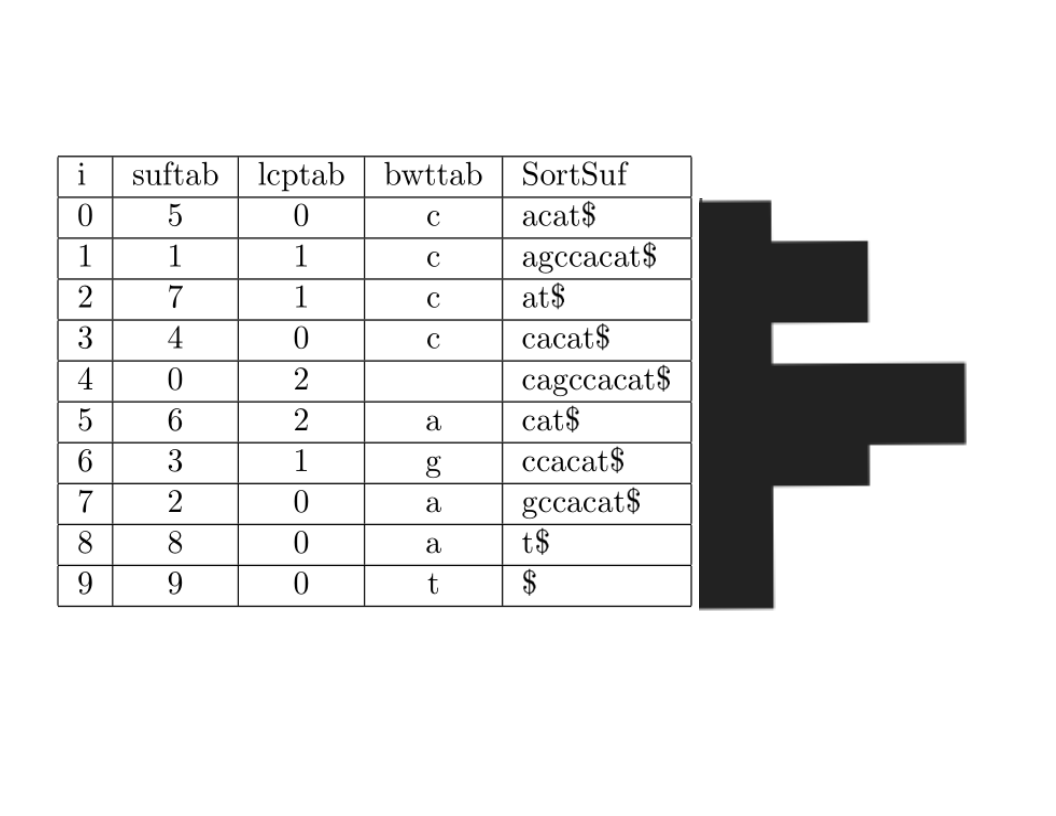
\includegraphics[width=\textwidth]{local_maxima.png}
%TODO: fix with figures

LCP-intervals can be embedded into each other, specifically, an
$\mathcal{k}-[i..j]$ is embedded in $\mathcal{l}-[k..l]$ iff $k \le i
\le j \le l$ and $\mathcal{k}<\mathcal{l}$.

Due to this, the enhanced suffix array of a string implicitely contains
a data structure called the LCP-interval tree. The root of the tree
contains information on the 0-interval: $0-[0..n]$ with $n=|S|$. The
leaves are the 1-intervals, each containing the starting and ending
position of the corresponding LCP interval.

The LCP-interval tree is just the suffix tree (\citealt{weiner1973linear})
without leaves, and its traversal enables linear time solutions to some
string matching problems using the enhanced suffix array.

The LCP-interval tree is not saved in memory, but reconstructed
by using the suffix array and the LCP array during execution
(\citealt{abouelhoda2002enhanced}).

%Tree bottom-up traversal is from the root to the leaves,
%top-down is the other way around

\section*{Different String Matching Problems}

A plethora of different string matching problems have been identified
by computer scientists, for many of which suffix arrays and enhanced
suffix arrays are useful.

\citealt[pg. 2]{abouelhoda2004replacing} summarizes suffix tree applications
from \citealt[chap. 2]{gusfield1997algorithms} and classify them after their
type of tree traversal.

\subsection*{Exact String Matching}

\subsubsection*{Description}

Give a string $S$ of length $n$ and a string $T$ of length $m$ with $m
\le n$ both using them same alphabet $\Sigma$, the exact matches of $T$
in $S$ is the set of indices $I=\{i_1, \ldots, i_k\}$ for which holds
that $\forall i \in I: S[i..i+m]=T$.

In other words, $I$ is the set of indices where $T$ is a substring in $S$.

\subsubsection*{Suffix Array Algorithm}

\citealt{manber1993suffix} describes an exact string matching algorithm
that runs in ${\cal{O}}(m \log n)$ time and constant space.

Their proposed algorithm uses binary search to sequentially find
the first (smallest) index $L_{W}$ and the last (biggest) index
$R_{W}$ in $\hbox{suftab}$ so that $S[\hbox{suftab}[L_{W}]]$ and
$S[\hbox{suftab}[R_{W}]]$ have the prefix $T$.

First, it searches $L_{W}$ using binary search on the whole array
$\hbox{suftab}$ and then uses $L_{W}$ as a left boundary to find $R_{W}$,
again by binary search.  Using $L_{W}$ as a left boundary improves
runtime as opposed to two independent searches over the whole array,
although the latter might be easier to parallelize.

\subsubsection*{Extended Suffix Array Algorithm}

\citealt{manber1993suffix} then propose a speed improvement based on
longest common prefixes that reduces the runtime to ${\cal{O}}(m + \log
n)$. Their method attempts to reduce the number of single-character
comparisons by only comparing characters that occur after the longest
common prefix of $T$ and $S[M_{W}]$ ($M_{W}$ being the index in the
middle between $L_{W}$ and $R_{W}$).

\citealt[p. 152]{gusfield1997algorithms} describes another speed-up
called the super-accelerant, which uses LCP-arrays to in practice reduce
runtime even further. It doesn't improve worst-case time complexity.

%They then go on to explain a more complicated method,
%and Gusfield expands on their work on pg. 152 (84 in the PDF).

I have not come across a proposal to use interpolation search first
described in \citealt{perl1978interpolation} to search the suffix array
with an improved ${\cal{O}}(\log \log n)$ runtime. This perhaps stems
from the fact that interpolation search assumes uniform distribution of
the alphabet, and has a worst-case runtime of ${\cal{O}}(n)$. It still
might be useful to empirically test speed differences in binary and
interpolation search.

\subsection*{Supermaximal and Maximal Repeats}

Enhanced suffix arrays were first designed to solve problems
in genome analysis, especially finding segmental duplications
(\citealt{lander2001initial}). Due to this, many algorithms have been
devised for finding different kinds of repeated substrings in a string
$S$.

\subsubsection*{Description}

Two substrings $S_1=S[i_1..j_1]$ and $S_2=S[i_2..j_2]$ are called a
repeated pair if $S_1=S_2$ and $i_1 \ne i_2$ and $j_1 \ne j_2$.  $S_1$
and $S_2$ are furthermore a maximal repeat iff $S[i_1-1] \ne S[i_2-1]$
and $S[j_1+1] \ne S[j_2+1]$. A supermaximal repeat is a maximal repeat
that does not occur as a substring of another maximal repeat.

Let $S_a$ and $S_b$ be two distinct strings over $\Sigma$. Let $\#
\not \in \Sigma$ be a character. Then a maximum unique match (MUM) is
a supermaximal repeat $((i_a, j_a)(i_b, j_b))$ of $S_a\#S_b$ so that
$j_a<|S_b|$ and $i_b>|S_a|$.

For example, the string "xabyabwabyz" contains the maximal repeat "ab"
(at positions $((1,2),(4,5))$ and $((4,5)(7,8))$) and the maximal repeat
"aby" at positions $((1,3),(7,9))$, as well as the supermaximal repeat
"aby" as positions $((1,3),(7,9))$. Note that the set of supermaximal
repeats is a subset of the set of maximal repeats.

\subsubsection*{Enhanced Suffix Array Algorithm for Finding Supermaximal Repeats}

Finding supermaximal repeats using an enhanced suffix array is
comparatively simple; the process can be visualized as finding
local maxima in $\hbox{lcptab}$  with pairwise distinct values in
$\hbox{bwttab}$.

\begin{algorithmic}
\State $\hbox{maxstart} \gets 0$
\State $\hbox{result} \gets \emptyset$
\For {$i$ in $0..n-1$}
	\If {$\hbox{lcptab}[i]>\hbox{lcptab}[i-1] \hbox{ and } i>0$}
		\State $\hbox{maxstart} \gets i$
	\ElsIf {$\hbox{lcptab}[i]<\hbox{lcptab}[i-1]$}
		\State $\hbox{preceding} \gets \emptyset$
		\For{$j$ in $\hbox{maxstart}..i-1$}
			\If {$\hbox{bwttab}[j] \in \hbox{preceding}$}
				\State \textbf{break}
			\EndIf
			\If {j=i-1}
				\State $\omega \gets S[\hbox{suftab}[i-1]..\hbox{suftab}[i-1] +\hbox{lcptab}[i-1]]$
				\State $\hbox{result} \gets \hbox{result} \cup \{(\omega, \hbox{maxstart}, i-1)\}$
			\EndIf
			\State $\hbox{preceding} \gets \hbox{preceding} \cup \hbox{bwttab}[j]$
		\EndFor
	\EndIf
\EndFor
\end{algorithmic}

This algorithm runs in $\mathcal{O}(n)$ time and is described first by
\citealt{abouelhoda2002enhanced}.

\subsubsection*{Finding Maximum Unique Matches}

Finding MUMs is just a special case of finding supermaximal repeats:

\begin{itemize}
\item The enhanced suffix array of $S_a\#S_b$ is generated
\item The algorithm for finding supermaximal repeats is executed
\item The set of supermaximal repeats is scanned for instance where $j_a<|S_b|$ and $i_b>|S_a|$
\end{itemize}

This algorithm also runs in $\mathcal{O}(n)$ time ($n=|S_a\#S_b|$).

While this is theoretically good, in practice the construction
of the enhanced suffix array for the two strings provides
some hurdles. Especially in the case of sequence assembly
(\citealt{myers2000whole}), where the maximum unique matches of sometimes
tens of thousands of reads have to be assembled, re-constructing the
enhanced suffix arrray for each pair of reads can be computationally
quite intensive. \citealt{salson2010dynamic} describes techniques for
updating modified suffix arrays and LCP arrays, which could be a useful
starting point for finding methods of combining enhanced suffix arrays
of concatenated strings.

\subsubsection*{LCP-interval tree Traversal}

\subsubsection*{Enhanced Suffix Array Algorithm for Finding Maximal Repeats}

\section*{Construction}

\section*{Comparison}

\section*{Applications}

%REPuter
%vmatch
%MUMmer

\section*{Conclusion}

\bibliographystyle{plainnat}
\bibliography{sources}

\end{document}
